
\subsection{Copulae}\label{subsec:copulae}
To capture different aspects of the dependence structure, we consider
a set of different copulas, which are layed
  out in detail below. These are the Gaussian-, $t$-, Frank-,
Gumbel-, Clayton-, mixture, NIG factor, and Plackett-copula. 

As this hedging backtest concerns only portfolios with two assets, we
focus on the bivariate version of each copula and bivariate copula
measures, such as Kendall's $\tau_K$ and Spearman's $\rho_S$. 

\subsubsection{Copula measures}

Kendall's $\tau$ and Spearman's $\rho$ are measures of association in
terms of concordance, see \cite{kruskal1958ordinal}. \natp{\em [A
  number of definitions follow. It usually helps the reader if they
  are put in a definition block rather than just flowing with the text.]}
Let $(x_i, y_i)$ and $(x_j, y_j)$ denote two realisations of a
vector $(X, Y)$ of continuous random variables. 
A pair of observations is concordant if $x_i<x_j$ and $y_i < y_j$, discordant if
$x_i>x_j$ and $y_i < y_j$ or if $x_i<x_j$ and $y_i>y_j$. \natp{\em
  [What about the case $x_i>x_j$ and $y_i>y_j$?]}
For a bivariate random variable of $n$ observations, there are
$\binom{n}{2}$ distinct pairs. \natp{\em [I struggled with
  understanding what ``distinct pairs'' refers to, but found the
  answer in Nelsen. Perhaps add a little more test. Also, as this
  paragraph seems to be taken directly from Nelsen, it {\bf must} be
  cited accordingly!]}


Let $c$ denote the number of concordant pairs, and $d$ the number of
discordant pairs. 
Kendall's tau is defined as follows: \citep{Nelsen1999}
\begin{equation*}
\tau_K := \frac{c-d}{c+d} = \frac{c-d}{\binom{n}{2}}. 
\end{equation*}

Let $F_X$ and $F_Y$ be the cdfs of $X$ and $Y$ respectively, Spearman's
$\rho$ is \natp{\em [These are two sentences, so please separate them
  into two sentences. Also, formulas belong syntactically to the
  sentence, so if they end the sentence, there should be a full stop.]}
\begin{equation*}
\rho_S := 12\E (F_X(X)F_Y(Y))-3. 
\end{equation*}
\natp{\em [Is there a particular reason to switch between sample and
  population versions?]}

Upper tail dependence is defined as \natp{\em [Typeset terms that are
  defined, e.g.\ upper tail dependence, in italics.]}
\begin{equation*}
\lambda_U :=  \lim_{q
  \rightarrow 1^-} \p\{X > F_{X}^{(-1)}(q)|Y > F_{Y}^{(-1)}(q)\};
\end{equation*}

Lower tail dependence is defined as
\begin{equation*}
\lambda_L :=  \lim_{q \rightarrow 0^+} \p\{X \leq F_{X}^{(-1)}(q)|Y
\leq F_{Y}^{(-1)}(q)\}. 
\end{equation*}
Furthermore, we denote the Fr{\'e}chet-Hoeffding lower bound by
$\bm{W}$, the product copula by $\bm{\Pi}$, and the Fr{\'e}chet-Hoeffding
upper bound by $\bm{M}$. They represent cases of perfect negative
dependence, independence, and perfect positive dependence,
respectively. 
For further details, we refer readers to \citet{joe1997multivariate}
and \citet{Nelsen1999}; see also \citet{hardle2010copulis}. 

The symmetry property of copulae is also important for modelling financial data.
In particular, we are interested in radial symmetry among various
concepts of symmetry, see \citet{Nelsen1999}. \natp{\em [Why?]}

\begin{defn}
  Let $(U_1, ..., U_d)$ be random variables. \natp{\em [uniform on $[0,1]$?]}
  The random variables is radially symmetric if the joint cdf of
  $(U_1, ..., U_d)$ is same as the joint cdf of $(1-U_1, ..., 1-U_d)$
\end{defn}


\subsubsection{Gaussian and $t$ Copulae}\label{sec:ellpitical-copulae}

The Gaussian and $t$ copulae are dervived from Gaussian and $t$
distributions. As the Gaussian and $t$ distributions belong to the family
of elliptical distributions, their copulae belong to the family of
elliptical copulae. \natp{\em [I personally would remove the reference
  to the elliptical family, as this is not important for what is to
  come. If it must stay, then briefly explain what elliptical distributions
  are (``Empirical distributions are characterised by...''.]}

The bivariate Gaussian copula is defined as
\begin{align*}
  \bm{C}(u,v) &= \Phi_{2, \rho}\{\Phi^{(-1)}(u), \Phi^{(-1)}(v)\} \nonumber \\
              &= \int_{-\infty}^{\Phi^{(-1)}(u)}
                \int_{-\infty}^{\Phi^{(-1)}(v)}
                \frac{1}{2\pi\sqrt{1-\rho^2}}
                \exp{\left\{
                \frac{s^2-2\rho st+t^2}{2(1-\rho^2)}
                \right\}} \dd s\, \dd t,\quad, u,v\in [0,1],
\end{align*}
where $\Phi_{2, \rho}$ is the bivariate Normal cdf
with zero mean, unit variance, and correlation coefficient $\rho$, and
$\Phi^{(-1)}$ is the quantile function of the univariate standard normal
distribution.
The Gaussian copula is fully specified by the correlation parameter $\rho$. \footnote{
The symbol $\rho$ is used to denote both the correlation parameter as
well as a general risk measure. However, it will be clear from the
context, what $\rho$ refers to.}
Like all elliptical copulas, it is symmetric. \natp{\em [Remove
  reference to elliptic copula.]}
It has no tail dependence, which, in a finance context, implies that
it often underestimates tail risk.  

The Gaussian copula density is
\begin{equation*}
  \bm{c}_\rho(u,v) = \frac{\bm{\varphi}_{2,\rho}\{\Phi^{(-1)}(u), \Phi^{(-1)}(v)\}}
                     {\varphi\{\Phi^{(-1)}(u)\} \cdot \varphi\{\Phi^{(-1)}(v)\}} 
                  = \frac{1}{2\pi\sqrt{1-\rho^2}}\exp\left\{
                     -\frac{u^2 - 2\rho uv + v^2}{2(1-\rho^2)}
                     \right\},
\end{equation*}
where $\bm{\varphi}_{2,\rho}(\cdot)$ is the pdf corresponding to
$\Phi_{2, \rho}$, and $\varphi(\cdot)$ the standard normal
pdf. \natp{\em [I think the abbreviations cdf and pdf where not
  introduced. Please double-check.]}

To illustrate the various copulae and their differences,
Figure~\ref{fig:copulaeScatterPlot} shows scatter plots of random
samples of each of the copulae treated. 
\begin{figure}[t]
    \centering
  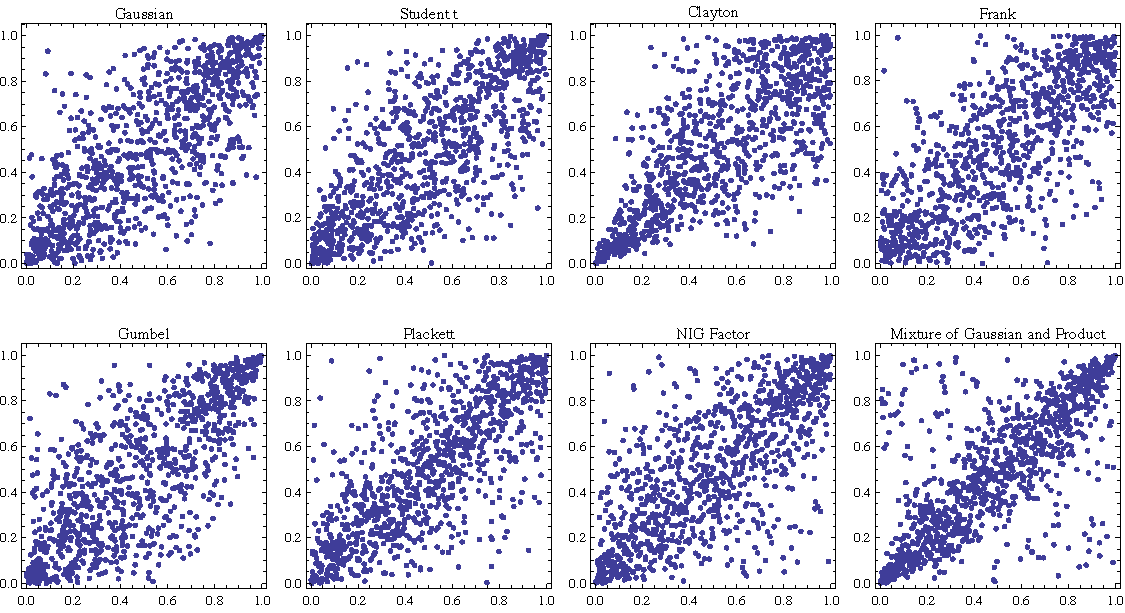
\includegraphics[width=\textwidth]{_pics/copulas_scatterplots.pdf}
  \caption{Scatterplots of samples drawn from various copulae. All
    copulae are calibrated to Spearman's $\rho$ of 0.75 before
    sampling.}\label{fig:copulaeScatterPlot} 
\end{figure}

Kendall's $\tau_K$ and Spearman's $\rho_S$ of the bivariate Gaussian copula are
    \begin{align*}
        \tau_K(\rho) = \frac{2}{\pi}\arcsin\rho
        \end{align*}
    \begin{align*}
        \rho_S(\rho) = \frac{6}{\pi}\arcsin\frac{\rho}{2}.
        \end{align*}

The $t$-copula has the form
\begin{multline*}
        \bm{C}(u,v) = \bm{T}_{2, \rho, \nu}\{T^{(-1)}_\nu(u), T^{(-1)}_\nu(v)\}\\
        = \int_{-\infty}^{T^{(-1)}_\nu(u)}
               \int_{-\infty}^{T^{(-1)}_\nu(v)}
            \frac{\Gamma\left(\frac{\nu+2}{2}\right)}
            {\Gamma\left(\frac{\nu}{2}\right)\pi\nu\sqrt{1-\rho^2}}
             \left(
        1+\frac{s^2-2st\rho+t^2}{\nu}
        \right)^{-\frac{\nu+2}{2}}\, \dd s\, \dd t,
    \end{multline*}
where $\bm{T}_{2, \rho, \nu}$ denotes the 
bivariate $t$ cdf with dependence parameter $\rho$ \natp{\em [Is this
  Spearman's Rho? If so, then say so.]} and degrees of
freedom parameter $\nu$, $\nu>2$,
and where $T^{(-1)}_\nu(\cdot)$ is the quantile function of a standard
$t$ distribution with parameter $\nu$. 

Contrary to the Gaussian copula, the $t$-copula has a non-zero
tail dependence coefficient, which makes it more appropriate for
dependence modelling in finance. The Gaussian copula arises as
$\nu\rightarrow\infty$.

The copula density is
\begin{align*}
    \bm{c}(u,v) &= \frac{\bm{t}_{2, \rho, \nu}\{T^{(-1)}_\nu(u), T^{(-1)}_\nu(v)\}}
    {t_\nu\{T^{(-1)}_\nu(u)\}\cdot t_\nu\{T^{(-1)}_\nu(v)\}},
    \end{align*}
where $\bm{t}_{2,\rho, \nu}$ is the pdf of $\bm{T}_{2, \rho, \nu}$
and $t_\nu$ the density of standard $t$ distribution.

\natp{The $t$-copula and Gaussian copula with parameter $\rho$ have
  equal Kendall's $\tau$, a property shared by all so-called
  elliptical copulas \citep[see][and
references therein]{demarta2005t}. (was: 
Like all the other elliptical copulae, the $t$-copula's Kendall's
$\tau$ is identical to that of the Gaussian copula \citep[see][and
references therein]{demarta2005t}.)}


\subsubsection{Archimedean copulae}\label{sec:archimedean-copula}
The family of Archimedean copulae forms a large class of copulae with
many convenient features.
% Contrary to elliptical copulas, which are derived from
% elliptical distributions.
Archimedean copulas are determined via a simple parametric form of the
dependence structure. A prominent feature is the ability to model
asymmetric dependence structures.  

In general, an Archimedean copula takes the form
\begin{align*}
    \bm{C}(u,v)= \psi^{(-1)}\{\psi(u), \psi(v)\},\quad u,v\in [0,1],
    \end{align*}
where $\psi:[0,1] \rightarrow [0,\infty)$ is a continuous, strictly
decreasing and convex function such that $\psi(1)=0$ \natp{\em [Where
  does $\theta$ come in?]} for any
permissible dependence parameter $\theta$. The function $\psi$ is 
called the generator, with $\psi^{(-1)}$ its inverse.

The {\em Frank copula\/} (B3 in \citet{joe1997multivariate}) takes the form
\begin{align*}
    \bm{C}_{\theta}(u,v) &= \frac{1}{\theta}
    \log \left\{
    1 + \frac{(e^{-\theta u}-1)(e^{-\theta v}-1)}{e^{-\theta}-1}
    \right\}, \quad u,v\in [0,1],
    \end{align*}
    with $\theta \in [0, \infty]$ the dependence parameter. It is a
    radially symmetric copula and cannot produce any tail
    dependence. The following parameters correspond perfect dependence
    and independence: $\bm{C}_{-\infty} = \bm{M}$, $\bm{C}_1 = \bm{\Pi}$,
    and $\bm{C}_\infty = \bm{W}$. The copula density is
    \begin{align*}
      \bm{c}_{\theta}(u,v)
      &= \frac{\theta e^{\theta(u+v)(e^\theta-1)}}
        {\left\{e^\theta-e^{\theta u}-e^{\theta v}+e^{\theta (u+v)}\right\}^2}.
    \end{align*}
    The Frank copula has Kendall's $\tau$ and Spearman's $\rho$ as follow:
\begin{align*}
    \tau_K(\theta) = 1-4\frac{D_1\{-\log(\theta)\}}{\log(\theta)},
    \end{align*}
and
\begin{align*}
    \rho_S(\theta) = 1-12\frac{D_2\{-\log(\theta)\} - D_1\{\log(\theta)\}}{\log(\theta)},
    \end{align*}
where $D_1$ and $D_2$ are the Debye function of order 1 and 2, with
the Debye function defined as $D_n =
\frac{n}{x^n}\int_0^x\frac{t^n}{e^t-1}dt$. \natp{\em [Please find a
  reference for the Debye function. A good candiate is the Handbook by
  Abramowitz Stegun.]}

The {\em Gumbel copula\/} (B6 in \citet{joe1997multivariate}) has
distribution function
\begin{equation*}
  \bm{C}_{\theta}(u,v) = \exp{-\{ (-\log(u))^\theta +(-\log(v))^\theta 
    \}^{\frac{1}{\theta}}},
\end{equation*}
where $\theta \in [1,\infty)$ is the dependence parameter.
It has upper tail dependence with dependence parameter $\lambda^U
= 2-2^{\frac{1}{\theta}}$ and displays no lower tail dependence. 
    
While the Gumbel copula cannot model perfect counter-dependence
\citep{Nelsen2002}, $\bm{C}_{1} = \bm{\Pi}$ models independence, 
and $\lim_{\theta\rightarrow\infty} \bm{C}_\theta = \bm{W}$ models
perfect dependence. The copula density takes the form
%\begin{align}
%        f
%    \end{align}
  \begin{equation*}
    \tau_K(\theta) =\frac{\theta-1}{\theta}. 
   \end{equation*}

The {\em Clayton copula\/} takes the form
\begin{equation*}
  \bm{C}_{\theta}(u,v) = \left\{
    \max(u^{-\theta}+v^{-\theta}-1,0)\right\}^{-\frac{1}{\theta}},
\end{equation*}
where $\theta \in (-\infty, \infty)$ is the dependence parameter.
The Clayton copula, by contrast to Gumbel copula,
generates lower tail dependence with $\lambda^L =
2^{-\frac{1}{\theta}}$, but cannot generate upper tail dependence.
Moreover, $\lim_{\theta\rightarrow -\infty} \bm{C}_\theta = \bm{M}$, $\bm{C}_0 =
\bm{\Pi}$, and $\lim_{\theta\rightarrow\infty} \bm{C}_\theta = \bm{W}$. 
Kendall's $\tau$ of the Clayton copula is given by 
\begin{align*}
    \tau_K(\theta) =\frac{\theta}{\theta+2}.
    \end{align*}

\subsubsection{Mixture Copula}\label{sec:mixture-copula}
The mixture copula is a linear combination of copulae. 
The distribution of a 2-dimensional random variable
$\bm{X}=(X_1,X_2)^\top$ is written as linear combination of $K$
copulae 
\begin{equation*} 
    \bm{C}(u,v)= \sum_{k=1}^K p^{(k)} \cdot \bm{C}^{(k)}\{F^{(-1)}_{X_1}(u),
    F^{(-1)}_{X_2}(v); \bm{\theta^{(k)}}\}, \quad u,v\in [0,1].
  \end{equation*}
  \natp{Here, $\bm{\theta^{(k)}}$ refers to the parameters of the
    $k$-th copula.} Likewise, the copula density is a linear
    combination of copula densities 
\begin{align*}
    \bm{c}(u,v)= \sum_{k=1}^K p^{(k)} \cdot \bm{c}^{(k)}\{F^{(-1)}_{X_1}(u),
    F^{(-1)}_{X_2}(v); \bm{\theta^{(k)}}\}.
    \end{align*}

\natp{\em
  [I think the statement below can go without a formal proof. Here is
  a suggestion].}

   
While Kendall's $\tau$ of the mixture copula is not known in closed form,
Spearman's $\rho$ is easily derived as 
\begin{equation*}
  \rho_S = \sum_{k=1}^K p^{(k)} \cdot \rho_S^{(k)}. 
\end{equation*}

\natp{\em [Old text below.]}

While Kendall's $\tau$ of the mixture copula is not known in closed form,
Spearman's $\rho$ is specified by the following statement. 
\begin{proposition}
  Let $\rho_S^{(k)}$ be Spearman's $\rho$ of the $k$-th component
  Spearman's $\rho$ of the mixture copula is given by 
  \begin{align*}
        \rho_S = \sum_{k=1}^K p^{(k)} \cdot \rho_S^{(k)}.
        \end{align*}
    \end{proposition}

\begin{proof}
  Since Spearman's $\rho$ is defined as \citep{Nelsen1999}
  \begin{equation*}
    \rho_S = 12 \int_{\mathbb{I}^2} \bm{C}(s,t) ds dt - 3,
  \end{equation*}
  Spearman's $\rho$ of the the mixture copula is given by summation
  of the components 
  \begin{align*}
    \rho_S = 12 \int_{\mathbb{I}^2} \sum_{k=1}^K p^{(k)} \cdot
    \bm{C}^{(k)}(s,t) ds dt - 3. 
  \end{align*}
\end{proof}
\natp{\em [Continue here.]}

An example of a mixture copula is the Fr\'echet class of copulae, which
are given by convex combinations of $\bm{W}$, $\bm{\Pi}$, and $\bm{M}$
\citep{Nelsen1999}.  

We use a mixture of Gaussian and independence copulae in our analysis,
i.e., 
\begin{equation*}
  \bm{C}(u,v) = p\, \bm{C}^\text{Gaussian}(u,v) + (1-p)(uv),\quad p\in (0,1),
\end{equation*}
with corresponding density 
\begin{equation*}
  \bm{c}(u,v) = p\, \bm{c}^\text{Gaussian}(u,v) + (1-p).
\end{equation*}

This mixture models the amount of ``random noise'' that appears in the
dependence structure. In the hedging exercise, the
``random noise'' adds an unhedgable component to the two-asset
portfolio, whose weight $(1-p)$ is calibrated from market
data. \natp{\em [Is it clear that the unhedgable part is more than the
  ``random noise''?]}

\subsubsection{NIG factor copula}

The {\em normal inverse Gaussian (NIG)\/} distribution, introduced by
\citep{BarndorffNielsen1997}, has density function
\begin{equation*}
  g(x; \alpha,\beta, \mu, \delta) = \frac{\alpha}{\pi} \e^{\delta
    \sqrt{\alpha^2-\beta^2} -\beta\mu} \frac{1}{q((x-\mu)/\delta)}
  K_1\left[\delta \alpha q\left(\frac{x-\mu}{\delta}\right) \right]
  \e^{\beta x},\quad x>0,
\end{equation*}
where $q(x) = \sqrt{1+x^2}$ and where $K_1$ is the modified Bessel
function of third order and index $1$. The parameters satisfy $0\leq
|\beta|\leq \alpha$, $\mu\in \R$ and $\delta>0$. The parameters have
the following interpretation: $\mu$ and $\delta$ are location and
scale parameters, respectively, $\alpha$ determines the heaviness of
the tails and $\beta$ determines the degree of asymmetry. If
$\beta=0$, then the distribution is symmetric around $\mu$.

The moment-generating function of the NIG distribution is given by
\begin{equation*}
  M(u; \alpha, \beta, \mu, \delta) = \exp\left( \delta
    \left(\sqrt{\alpha^2-\beta^2} - \sqrt{\alpha^2 - (\beta +
        u)^2}\right) + \mu u\right). 
\end{equation*}
As a direct consequence, moments are easily calculated with the
expectation and variance of the NIG distribution being
\begin{align*}
  \mathbb E X &= \mu +
                \frac{\delta \beta}{\sqrt{\alpha^2-\beta^2}}
  \end{align*}
\begin{align} \label{eq:5}
  \text{Var}(X) &= \frac{\alpha^2\delta}{(\alpha^2-\beta^2)^{3/2}}.
\end{align}


The $\text{NIG}(\alpha, \beta, \mu\, \delta)$ distribution belongs to
the class of so-called {\em normal
variance-mean mixture distributions},  (see Section 3.2 of 
\citep{McNeil2005}): $X$ follows an
$\text{NIG}(\alpha,\beta,\mu,\delta)$ distribution if $X$ conditional
on $W$ follows a normal distribution with mean $\mu+\beta W$ and
variance $W$, i.e., 
\begin{equation*}
  X|W\stackrel{\mathcal L}\sim \Ncdf(\mu + \beta W, W),
\end{equation*}
where $W$ follows an {\em inverse Gaussian distribution}, denoted by
$\text{IG}(\delta, \sqrt{\alpha^2-\beta^2})$.

It is easily seen from the moment-generating function that the NIG distribution is preserved under linear combinations, provided
the variables share the parameters $\alpha$ and $\beta$. For this
and other reasons, the NIG distribution is popular in many areas of
financial modelling; for example, it gives rise 
to the normal inverse Gaussian L\'evy process, which may be represented
as a Brownian motion with a time change.

In the setting here, we consider the {\em NIG factor copula}. This is
not directly derived from the multivariate NIG distribution, but
determined through a factor structure instead. The factor structure,
which 
was applied e.g.\ in \citep{Kalemanova2007} for calibrating CDO's,
gives additionaly flexibility as it does not force the components to
have a mixing variable $W$.
The following proposition introduces the NIG factor model and some of
its properties.
\begin{proposition}
  \label{prop:NIG}
  Let $Z\sim \text{NIG}(\alpha, \beta, \mu, \delta)$ and
  $Z_i\sim \text{NIG}(\alpha, \beta, \mu_i, \delta_i)$,
  $i=1,\ldots, n$ be independent NIG-distributed random
  variables. Then:
  \begin{enumerate}
  \item  $X_i = Z + Z_i\sim \text{NIG}(\alpha,\beta,\mu+\mu_i,
  \delta+\delta_i)$,
\item and 
  \begin{align}
    \text{Cov}(X_i,X_j) &= \text{Var(Z)},\nonumber\\
    \text{Corr}(X_i,X_j) &= \frac{\delta}{\sqrt{(\delta+\delta_i)
                           (\delta+\delta_j)}}. \label{eq:6}
  \end{align}
\end{enumerate}
\end{proposition}
\begin{proof}
  \begin{enumerate}
  \item This follows directly from the moment-generating function. 
  \item For the covariance,
    \begin{equation*}
      \text{Cov}(X_i,X_j)
      = \E[(Z+Z_i) (Z+Z_j)] - \E[Z+Z_i] \E[Z+Z_j]
      = \E[Z^2] -(\E Z)^2.
    \end{equation*}
    The correlation is determined directly from \ref{eq:5}.
  \end{enumerate}
\end{proof}

\natp{\em [Please clarify that $\circ$ refers to composition. Clean
  up notation, e.g.\ marginals can be denoted $F_F$ and $F_S$, Use
  just $C$ for the copula. What are $Z_1$ and $Z_2$? I don't find the
  formula in the paper mentioned. Also, where is the formula for
  Kendall's tau taken from?]}
 The NIG factor copula is obtained by transforming the margins to
uniforms (see Sklar's Theorem), giving (e.g.\
\citep{krupskii2013factor}):
\begin{equation*}
  C_{r^S, r^F}(F_{r^S}(r^S), F_{r^F}(r^F)) = \int_\mathbb{R}
  F_{Z_1}(F_{X_1}^{(-1)} \circ F_{r^S}(r^S) -z) \cdot
  F_{Z_2}(F_{X_2}^{(-1)} \circ F_{r^F}(r^F) -z) \cdot
  f_Z(z) dz.
  \end{equation*}
If the margins are continuous, then Spearman's rho of NIG factor
copula is 
\begin{equation*}
  \rho_S = 12 \int \int \int_{\mathbb{R}^3}
  F_{X_1}(x_1) \cdot
  F_{X_2}(x_2) \cdot
  f_{Z_1}(x_1-z) \cdot
  f_{Z_2}(x_2-z) \cdot
  f_Z(z) dx_1 dx_2 dz - \frac{1}{48}.
  \end{equation*}

% \begin{proof}
%   \begin{align}
%   \rho_S(r^S, r^F) &= \rho\{F_{r^S}(r^S), F_{r^F}(r^F)\} \\
%     &= \rho\{F_{X_1}(X_1), F_{X_2}(X_2)\} \\
%     &= 12 \cdot \mathbb{E}\{F_{X_1}(X_1) \cdot F_{X_2}(X_2) \} - \frac{1}{48}\\
%     &= 12 \cdot \int \int_{\mathbb{R}^2} F_{X_1}(X_1) \cdot F_{X_2}(X_2) dF_{X_1,X_2}(x_1,x_2)\\
%     \end{align}
%   Because
%   \begin{align}
%     F_{X_1,X_2}(x_1,x_2) &= \mathbb{P}(X_1 \leq x_1, X_2 \leq x_2)\\
%     &= \mathbb{P}(Z_1 \leq x_1 - Z, Z_2 \leq x_2 - Z) \\
%     &= \int_\mathbb{R}\mathbb{P}(Z_1 \leq x_1 - z) \cdot \mathbb{P}(Z_2 \leq x_2 - z) \cdot f_Z(z) dz,
%     \end{align}
%   so,
%   \begin{align}
%     \rho_S(r^S, r^F) = 12 \cdot \int \int \int_{\mathbb{R}^3} F_{X_1}(x_1) \cdot F_{X_2}(x_2) \cdot f_{Z_1}(x_1 -z) \cdot f_{Z_2}(x_2 -z) \cdot f_{Z}(z) dx_1 dx_2 dz -\frac{1}{48}
%     \end{align}
%   \end{proof}


\subsubsection{Plackett copula}\label{subsec:other-copula}
The Plackett copula has distribution functiono
\begin{align*}
    \bm{C}_{\theta}(u,v) &= \frac{1+(\theta-1)(u+v)}{2(\theta-1)}
                         - \frac{\sqrt{\{
    1+(\theta-1)(u+v)\}^2 - 4uv\theta(\theta-1)}}{2(\theta-1)},
\end{align*}
\natp{where $\theta$...}.
Spearman's Rho is given by 
\begin{align*}
    \rho_S(\theta) = \frac{\theta+1}{\theta-1} - \frac{2\theta \log
  \theta}{(\theta-1)^2}. 
    \end{align*}

The Placket copula possesses a special property, namely
the cross-product ratio is equal to the dependence parameter
\begin{equation} \label{eq:PlackettCrossProduct}
    % &\phantom{=}
    \frac{\p(U \leq u, V \leq v) \cdot \p(U > u, V > v)}
    {\p(U \leq u, V > v) \cdot \p(U > u, V \leq v)}\nonumber
    =
      \frac{\bm{C}_\theta(u,v)\{1-u-v+\bm{C}_\theta(u,v)\}}{\{u-\bm{C}_\theta(u,v)\}\{v-\bm{C}_\theta(u,v)}\nonumber 
    = \theta.
\end{equation}
In words, the dependence parameter is equal to the ratio of the 
number of concordance pairs and the number of discordance pairs of a 
bivariate random variable. 


%%% Local Variables:
%%% mode: latex
%%% TeX-master: "SRM"
%%% End:
